\chapter{Getting Started}

\section{Introduction}
	De CircuitPython omgeving is ontworpen voor beginners in software en elektronica. Voordat je met het CircuitPython bordje aan de slag kan moet het \'e\'en en ander worden ge\"installeerd en ge\"updatet. Adafruit heeft een beginners tutorial voor CircuitPython die je gaat doorlopen in ~\ref{sec:CircuitPythonTutorial}.%, maar de Adafruit Metro M4 Express heeft een WIFI module die eerst ge\"updatet moet worden.

%\section{Updaten van de WIFI module}
	
	%Als je Windows 7 gebruikt moet je eerst de nieuwste drivers installeren van de volgende link:\\
	%\url{https://github.com/adafruit/Adafruit_Windows_Drivers/releases}\\
	%Mac en Linux gebruikers hoeven geen drivers te installeren.\\
	
%Als je al eens code op de CIRCUITPY drive hebt gezet, maak dan een back-up, want het wordt overschreven door de code die je nu gaat uploaden. Als dit de eerste keer is dat je het bordje gebruikt kan je de back-up overslaan.\\
	
	%\noindent Download de  Metro\_M4\_WIFI\_ESP32\_Passthru.uf2 file van:\\
	%\url{https://learn.adafruit.com/upgrading-esp32-firmware/upgrade-an-airlift-all-in-one-board}\\
	
	
	%\noindent Zoek het reset knopje op je bordje. Het is een klein zwart knopje, te zien in figuur \ref{fig:ResetButton}. Druk twee keer op dit knopje om het bordje in de bootloader te zetten. Als het niet de eerste keer lukt, probeer het dan opnieuw. Het ritme moet goed zijn en dat kan een paar pogingen kosten. Als het is gelukt zal de RGB LED op het bordje rood knipperen en daarna groen blijven. Een nieuwe schijf genaamd bordnaamBOOT zal verschijnen als in figuur \ref{fig:Bootloader}, waar bordnaam een referentie naar de naam van je bord is.\\
	
%	\begin{figure}[!htb]
%		\center{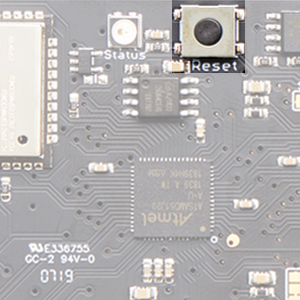
\includegraphics[width=0.3\linewidth]{figures/ResetButton.png}}
%		\caption{De reset knop}
%		\label{fig:ResetButton}
%	\end{figure}
	
	
%	\begin{figure}[!htb]
%		\center{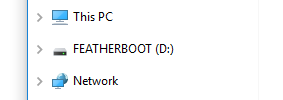
\includegraphics[width=0.6\linewidth]{figures/Drive.png}}
%		\caption{De micro-controller in bootloader}
%		\label{fig:Bootloader}
%	\end{figure}
	
%	\newpage\noindent Het bordje is nu in bootloader mode. Zoek de UF2 file die je net hebt gedownload en sleep het naar de BOOT schijf op je computer zoals in figuur \ref{fig:UF2}. De lichtjes knipperen nu opnieuw en de BOOT schijf verdwijnt.\\

%\footnotesize\noindent Originele bron: \url{https://learn.adafruit.com/upgrading-esp32-firmware/upgrade-an-airlift-all-in-one-board}
%\normalsize

%\begin{figure}[H]
%	\center{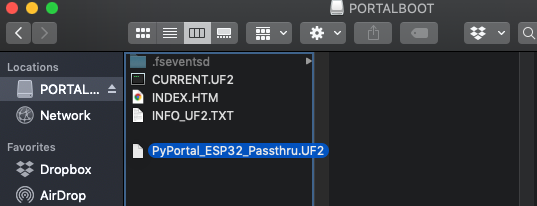
\includegraphics[width=\linewidth]{figures/UF2_install.png}}
%	\caption{Sleep de UF2 file naar de BOOT drive}
%	\label{fig:UF2}
%\end{figure}

\section{Welcome to CircuitPython tutorial}\label{sec:CircuitPythonTutorial}
	Alle andere benodigdheden om te starten met CircuitPython wordt behandelt in Adafruit's kennismaking tutorial. Doorloop Adafruits' \textbf{"Welcome to CircuitPython"} tutorial tot en met het kopje \textbf{"CircuitPython Libraries"} op:\\
	
	\url{https://learn.adafruit.com/welcome-to-circuitpython/} \\

Op deze website staat de basis van cirquit python, lees dit goed door. Download ook \href{https://codewith.mu/}{de Mu editor} zoals op de guide staat aangegeven. \\
	
	\url{https://codewith.mu/}


\section{Plotten met Mu editor}\label{sec:plotter}
In de Mu editor zit een ingebouwde plotter. Dit is erg handig om bijvoorbeeld sensordata direct te plotten. Om gebruik te maken van de plotter moet data in een tuple geprint worden. Open mu editor om dit te testen. Klik op Serial en Plotter bovenaan mu editor. Als het goed is ziet je scherm eruit als figuur~\ref{fig:SerialPlotter}. Als er een programma loopt, klik dan in het vak van de repl en doe ctrl+c om de code te stoppen en druk op een een willekeurige knop om in de repl te gaan. Print nu een paar tuples. Een tuple is een datastructuur dat normale haakjes () gebruikt. Type in de repl bijvoorbeeld de volgende commands, print((1,2)), print((3,2)), a=(0,0), print(a). Als het goed is zie je dan hetzelfde als in figuur~\ref{fig:TuplePlot}. Probeer ook \'e\'en getal te plotten door bijvoorbeeld print((4)) te typen. Als het goed is zie je niks gebeuren. Dit komt door een eigenaardigheid in python dat een enkel getal in een tuple geschreven moet worden als (4,) en niet (4) . Als je print((4,)) typt wordt de waarde wel geplot.

\begin{figure}[H]
	\center{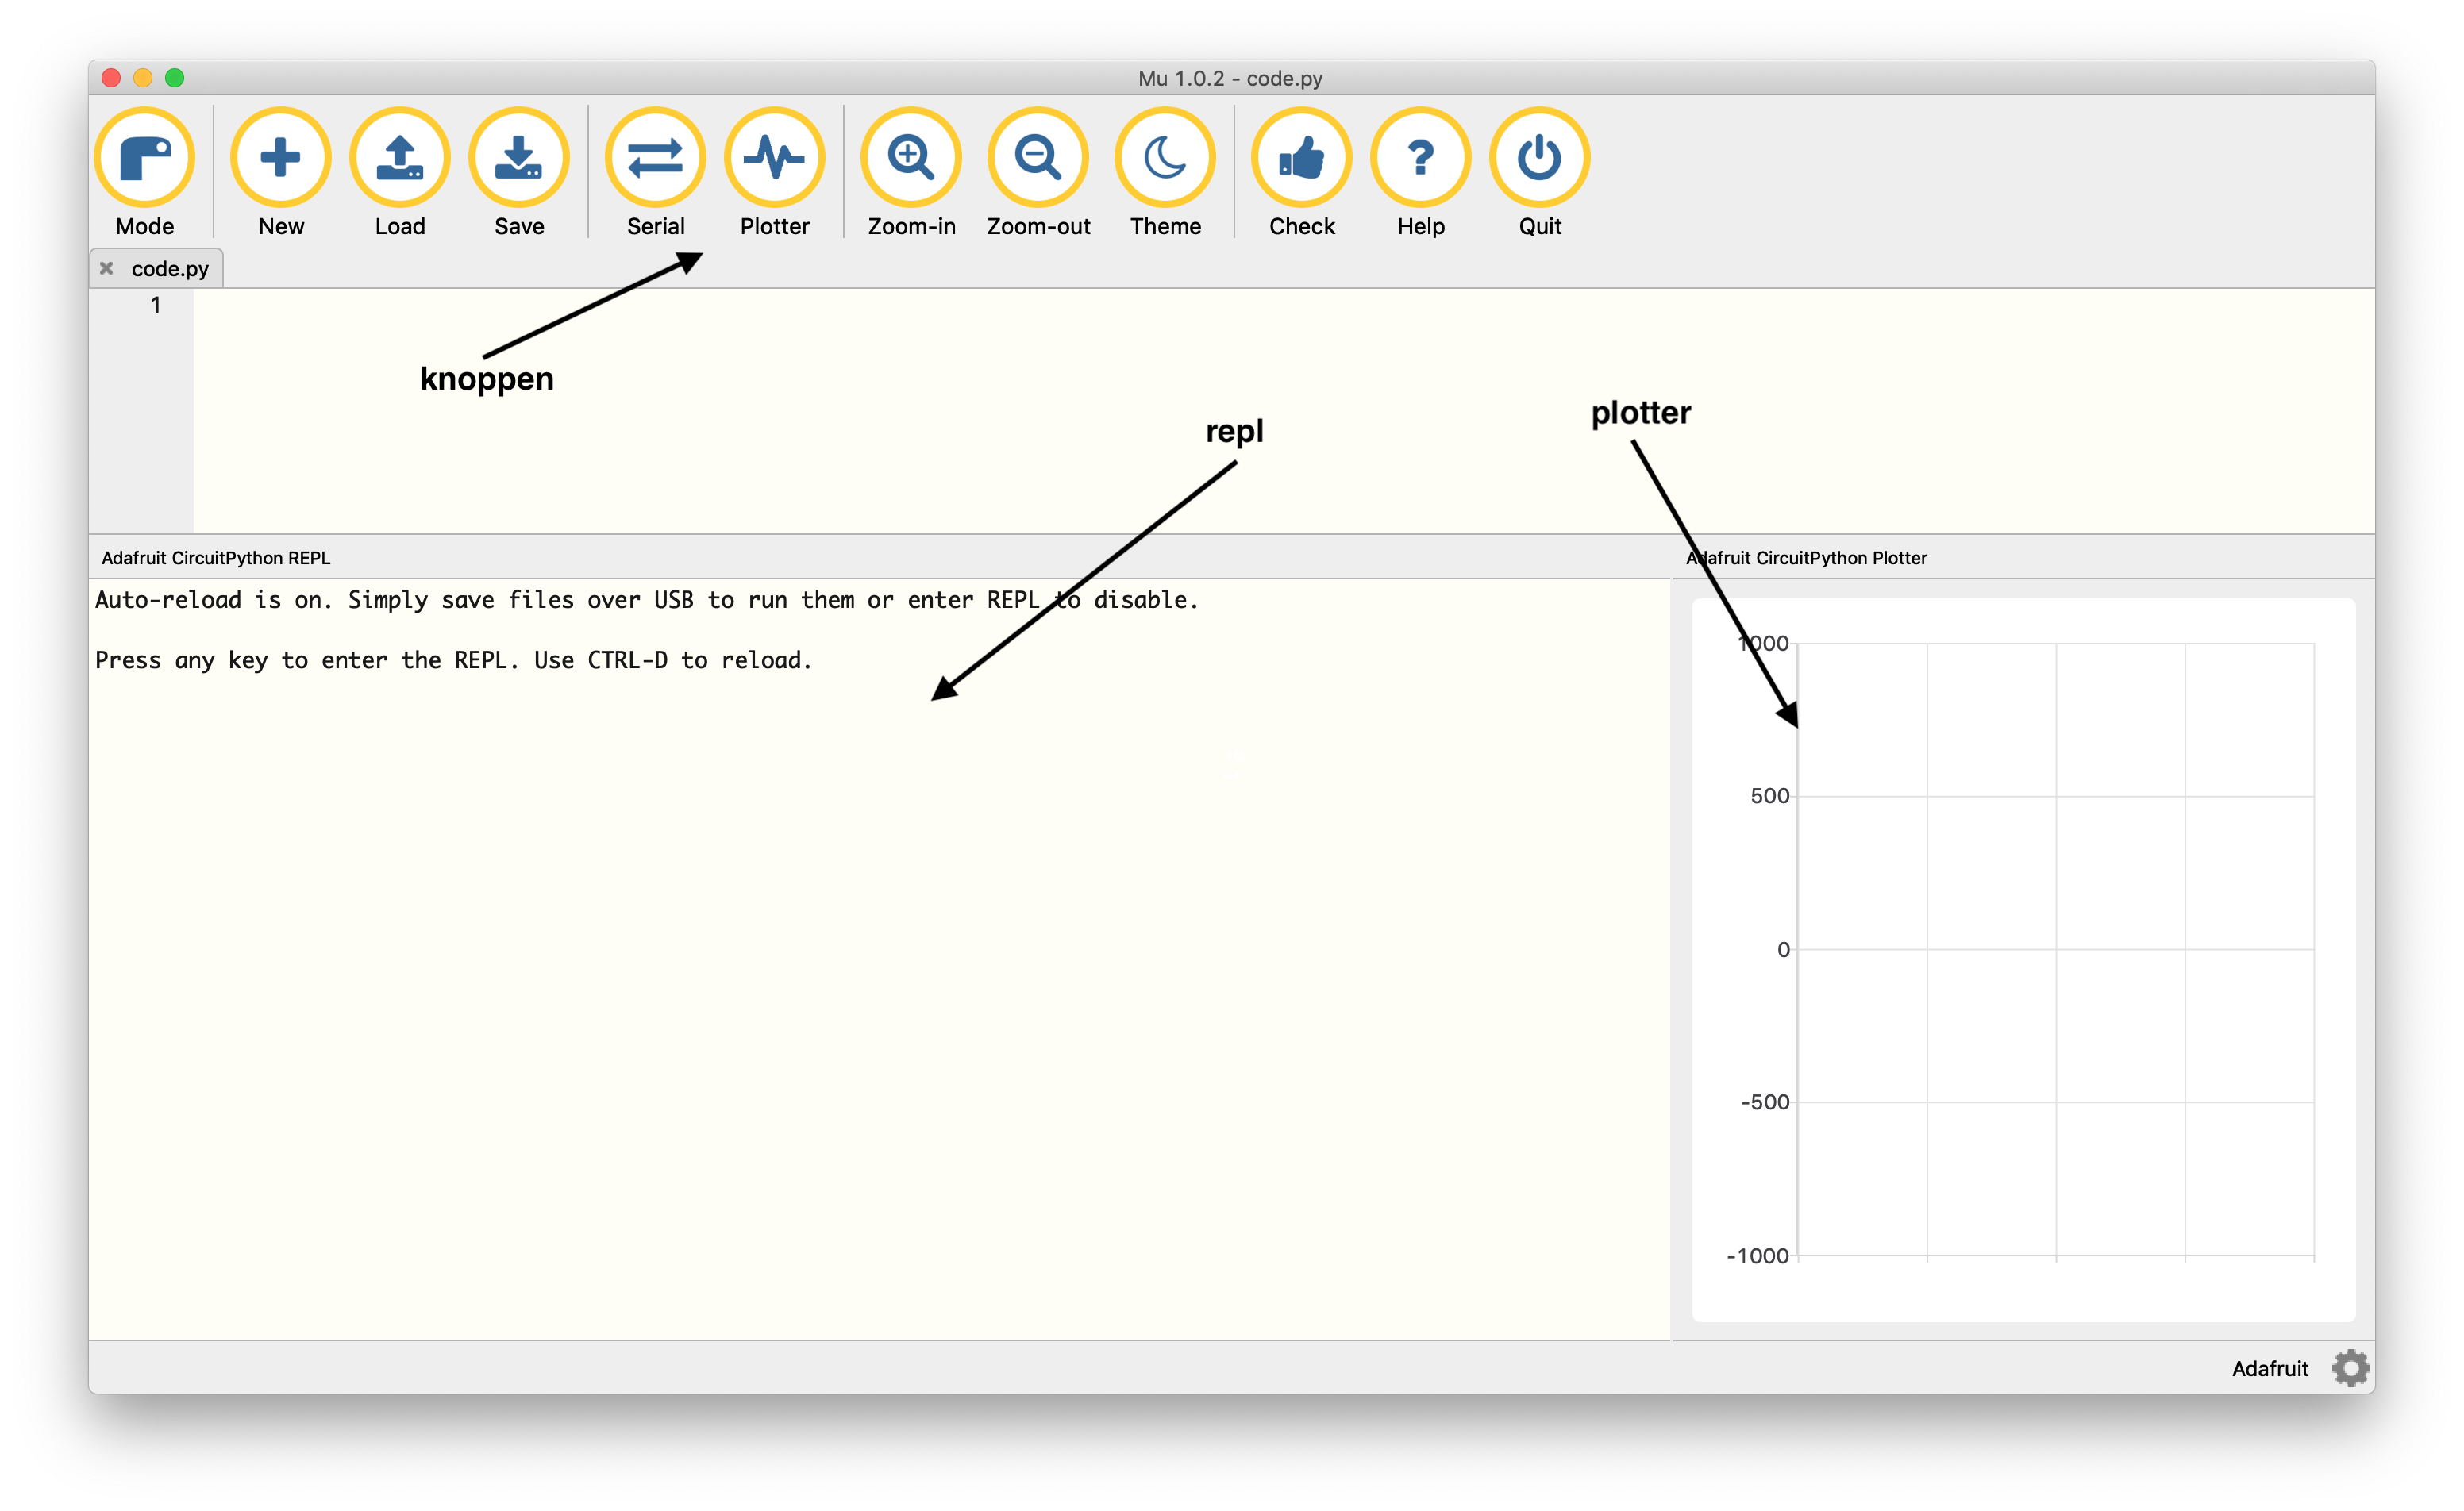
\includegraphics[width=0.9\linewidth]{figures/SerialPlotter.png}}
	\caption{Mu editor met de REPL en plotter open}
	\label{fig:SerialPlotter}
\end{figure}

\begin{figure}[H]
	\center{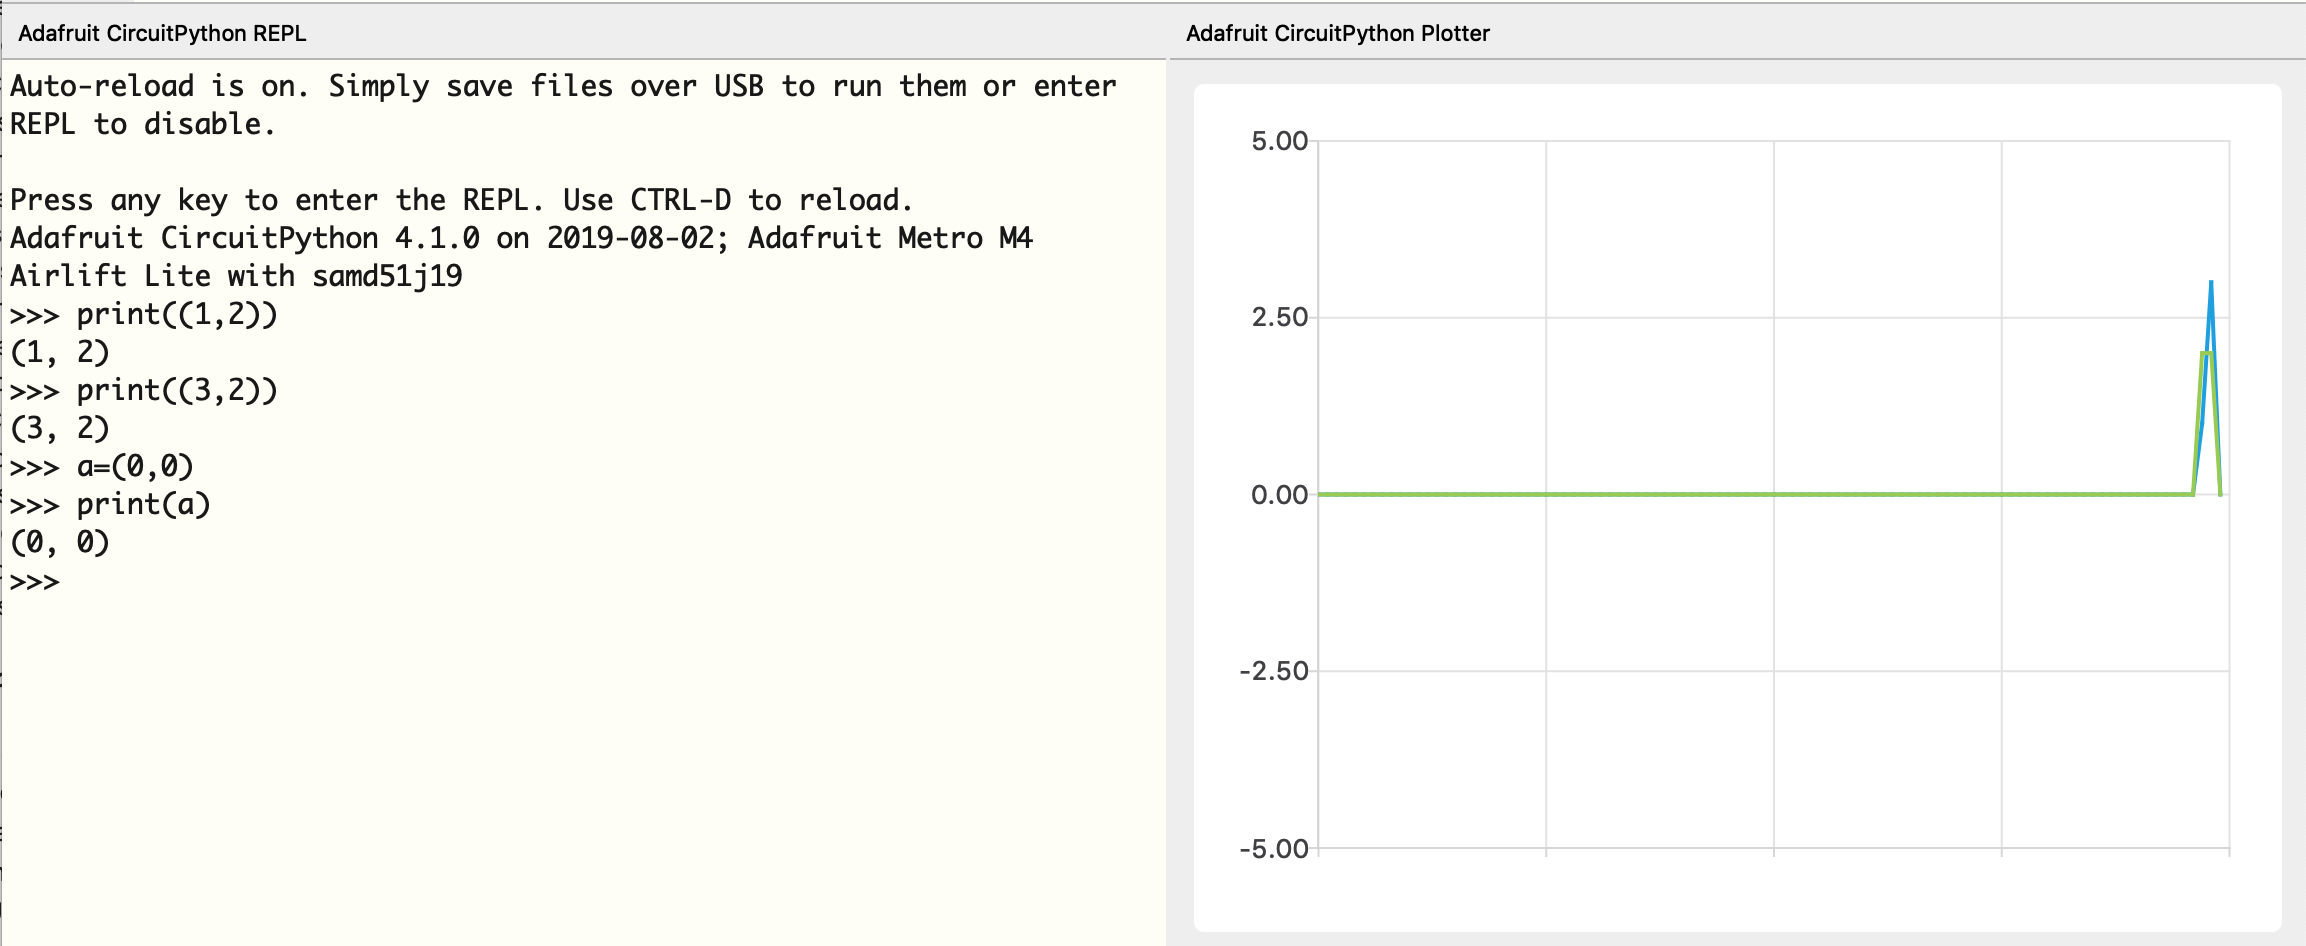
\includegraphics[width=0.9\linewidth]{figures/TuplePlot.png}}
	\caption{Plotten van tuples}
	\label{fig:TuplePlot}
\end{figure}


\url{https://learn.adafruit.com/make-it-graph-plot}

\newpage
\section{Een extra woord over bibliotheken}\label{sec:library}
In deze handleiding wordt gebruik gemaakt van de volgende bibliotheken:
\begin{itemize}
	\item adafruit\_bus\_device map
	\item adafruit\_esp32spi map
	\item adafruit\_hcsr04.mpy
	\item adafruit\_motor map
	\item neopixel.mpy
\end{itemize}

Haal de up-to-date bibliotheken uit adafruits library bundle en zet ze in de lib folder van je CIRCUITPY drive. De bundel is te downloaden op \\

\url{https://circuitpython.org/libraries}. \\

Let op, je kan niet alle bibliotheken op het bordje zetten, hiervoor is niet genoeg ruimte. Zet dus alleen de bibliotheken die je gebruikt op het bordje.


\section{Veilig omgaan met het bordje}\label{sec:VeiligOmgaan}
De bordjes kunnen kapot gaan als de pinnen op het bordje teveel stroom moeten leveren of als er teveel stroom het bordje instroomt. Het Adafruit Metro M4 Express bordje heeft een \SI{3.3}{\volt}, \SI{5}{\volt} en een $V_{in}$ output pin, te zien in figuur~\ref{fig:MetroM4}. Deze pinnen kunnen bij elkaar maximaal \SI{500}{\milli\ampere} leveren en kunnen gebruikt worden om je projectje te voorzien van stroom. Alle andere pinnen op het bordje zijn I/O pinnen en zijn niet bedoeld om zulke hoge stroom te leveren. In de datasheet van de ATSAM51D wordt een maximum van \SI{2}{\milli\ampere} per I/O pin aangegeven. Als je je hier niet aan houdt is het mogelijk dat componenten in het bordje doorbranden. Zie \url{https://www.alanzucconi.com/2016/09/17/how-to-destroy-an-arduino-board/} voor meer informatie over hoe je een bordje kapot kan maken.

\begin{figure}[!htb]
	\center{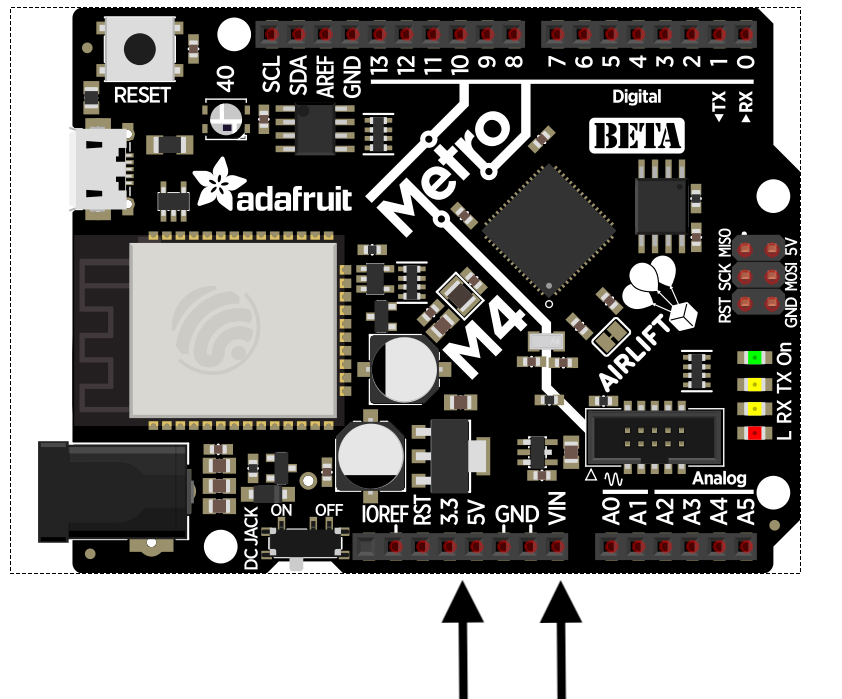
\includegraphics[width=0.8\linewidth]{figures/MetroM4.png}}
	\caption{De spanningsbronnen op de Metro M4 Express}
	\label{fig:MetroM4}
\end{figure}

\clearpage
\newpage

\section{Bordje updaten}

\begin{center}
    Let op: dit alleen uitvoeren als de docent hier om vraagt!
\end{center}

Het bordje kan ge\"{u}pdatet worden door het bordje in de bootloader modus te zetten en het update bestand erop te slepen. \\

Download eerst de update van de bootloader op de volgende link (onderaan op pagina). Let op download alleen se stabiele versie, dus geen alpha of beta builds. \\

\url{https://circuitpython.org/board/metro_m4_airlift_lite/} \\

Klik twee keer op reset om Het bordje in bootloader modus te zetten. Sleep vervolgens het update bestand (de nieuwe bootloader) op het bordje. Het bordje zal opnieuw opstarten. Na het updaten van de bootloader zal CirquitPython van het bordje zijn verdwenen, deze moet er dus opnieuw worden opgezet. Download op dezelfde pagina ook de laatste versie van CirquitPython, zet het bordje weer in bootloader modus en sleep het cirquitPython bestand naar de bootloader. Het bordje zal weer opnieuw opstarten. \\

Gefeliciteerd, je hebt nu de bootloader en CirquitPython ge\"{u}pdatet!

